\documentclass[12pt,a4paper]{article}
\usepackage{fontspec}
\setmainfont{Times New Roman}
\setmonofont{Courier New}
\usepackage{graphicx}
\usepackage[russian]{babel}
\usepackage{amsmath,amssymb,geometry,booktabs,longtable,hyperref}
\geometry{margin=22mm}
\emergencystretch=3em
\title{Система машинного зрения для анализа размеров замороженных углеводородных шариков}
\author{И. Л. Литвак}
\date{Раздел 1 итогового отчёта по НИР\\Рабочая редакция от 30 сентября 2026 года}
\begin{document}
\maketitle
\noindent\textbf{Основание.} Техническое задание к договору на выполнение НИР по разработке макета установки для изготовления твёрдых замороженных шариков из углеводородов для криогенных замедлителей нового перспективного источника нейтронов в ЛНФ ОИЯИ. Номер и дата договора в предоставленном ТЗ не заполнены.

\begin{abstract}
Разработано программное обеспечение измерения круговых проекций шариков по сохранённым видеозаписям. Реализованы обнаружение нескольких объектов, сопровождение, скалярная калибровка, оценка модельной неопределённости, построение распределений и экспорт результатов. Программный контур проверен модульными и интеграционными тестами и двумя наборами синтетических видеосцен. В ходе работы я опробовал подключение камеры. Погрешность измерений на реальном стенде и применимость модели к рабочей оптической среде предстоит установить экспериментально.
\end{abstract}
\clearpage
\tableofcontents
\clearpage

\section{Назначение и требования к системе}
Цель НИР состоит в подготовке научно-технического отчёта для разработки проекта технического задания на создание макета установки по изготовлению твёрдых шариков из углеводородов в жидком хладагенте. Состав результатов установлен техническим заданием и календарным планом к договору \cite{tz}.

Система машинного зрения предназначена для определения размеров шариков по изображениям, анализа распределения диаметров и документирования измерений. Полученные данные предполагается использовать при оценке качества изготовления шариков и экспериментальной проверке модели теплообмена. Для этой задачи я разработал программное обеспечение обработки видеозаписей и опробовал подключение камеры. Экспериментальные серии на автоматизированном макете к настоящей редакции отчёта не подготовлены.


Требования ТЗ к этому разделу включают описание оборудования и ПО, алгоритмов сегментации и калибровки, примеры исходных изображений и результатов обработки, распределение диаметров и оценку погрешности $\pm\Delta d$. В данной редакции представлены программные методы и синтетические результаты. Реальные исходные изображения, эталонные измерения и параметры комплектации должны войти в окончательную редакцию после получения материалов стенда.

\section{Система машинного зрения и программное обеспечение}
\subsection{Состояние аппаратной части}
Для системы машинного зрения я выбрал монохромную промышленную камеру Daheng MER2-231-41GM и опробовал её подключение. Модель указана в счёте ООО «МКОИ» № 382 от 26.09.2025 и в моей переписке по подбору объектива в ноябре 2025 года \cite{cameraorder,equipmentmail}. Камера оснащена CMOS-сенсором Sony IMX249 с глобальным затвором, имеет разрешение $1920\times1200$ пикселей, размер пикселя 5.86 мкм и паспортную частоту до 41 кадра/с. Интерфейс передачи данных --- GigE; питание --- 12--24 В постоянного тока \cite{daheng}. Паспортная частота не является измеренной частотой экспериментальной регистрации.

Для комплектации стенда я согласовал с поставщиком объектив, кольцевой осветитель, контроллер и механическую оснастку. В таблице приведены позиции счёта № 382 и счёта «Азимут Фотоникс» № 15022 от 20.11.2025 \cite{cameraorder,opticsorder}. На позиции второго счёта найден УПД № 78 от 19.02.2026; он содержит дату отгрузки, но поле даты приёмки в предоставленной копии не заполнено \cite{equipmentupd}. Поэтому состав закупочных документов и факт установки каждой позиции на стенде учитываются отдельно.

\begin{longtable}{p{60mm}p{72mm}}
\toprule
Оборудование & Назначение и параметры по документам\\
\midrule
\endhead
Daheng MER2-231-41GM & Монохромная камера, Sony IMX249, глобальный затвор, GigE; одна штука\\
HR25-7TP-8S & Кабель I/O камеры, восемь проводов, длина 3 м\\
Крепление NS & Крепление камеры к штативу, резьба 1/4 дюйма\\
\path{VT-LEM1214CB-H1} & Объектив Contrastech, 12 мм, F1.4, формат 1 дюйм, C-mount, номинально 5 Мп\\
\path{VT-C2CS} & Кольца C-mount толщиной 0.5, 1, 5, 10 и 20 мм\\
\path{VT-LT2-HR12076-90W} & Белый кольцевой осветитель с диффузором, 24 В; наружный диаметр 120 мм, внутренний 76 мм\\
\path{LT2-CB-1} & Кабель осветителя, длина 1 м\\
\path{VT-LT4-2420PWDC-2} & Двухканальный контроллер освещения, 24 В, 20 Вт\\
\path{GST25E12-P1J} & Адаптер MEAN WELL, 12 В, 25 Вт\\
Raylab RL-GT3 и RL-GT2 & Настольный кронштейн со струбциной и дополнительный двухрычажный держатель\\
\bottomrule
\end{longtable}

Получение оплаты заказа «Азимут Фотоникс» подтверждено письмом поставщика от 10.12.2025. В письме от 20.04.2026 поставщик уточнил, что заказанный метровый кабель подсветки поступил позднее; до этого был предоставлен временный кабель длиной 3 м \cite{equipmentmail}. Для протокола конкретного опыта следует указать фактически использованный кабель и схему монтажа. Данные о выбранной оптике и освещении дополняются настройками экспозиции, усиления, диафрагмы, частоты кадров, положения камеры и режимом контроллера. Эти настройки экспериментальной серии пока не зафиксированы в настоящем разделе.

Опробование подключения подтверждает выполнение подготовительного действия. Измерительная калибровка и погрешность определения диаметра должны подтверждаться отдельной эталонной серией. В текущей редакции численная точность системы не заявляется.

\subsection{Порядок проведения измерений}
Для подготовки экспериментальных серий я обновил руководство по стенду до версии 2.1 от 30.09.2026 \cite{manualv2}. В нём приведены порядок регистрации исходных видео, калибровка по одному эталонному треку, пакетная обработка нескольких объектов, состав экспортов и контроль качества. Новая редакция заменяет устаревшие программные процедуры инструкции от 02.04.2026. Полный текст новой редакции включён в приложение. Цель 0.01 мм из прежней инструкции не принимается за достигнутую точность; параметры геометрии и оптической среды проверяются для каждой серии.

\subsection{Устройство программного обеспечения}
Программа разработана на Python. Единая точка запуска \path{run_analysis.py} принимает путь к видеозаписи и параметры обработки из командной строки либо текстового файла конфигурации. Параметры включают режим пересчёта масштаба, диапазон диаметров, шаг обработки кадров, параметры детекции и входные оценки неопределённости \cite{code}.

Рабочий программный контур использует OpenCV для чтения видео и обработки изображений, NumPy для вычислений, SciPy для глобального сопоставления объектов и Matplotlib для графиков. На компьютере, использованном для программной проверки 30 сентября 2026 года, установлены Python 3.11.5, OpenCV 4.12.0, NumPy 2.2.6 и Matplotlib 3.10.3. Это версии среды текущей проверки, а не установленная конфигурация будущего экспериментального стенда. Файл зависимостей проекта содержит названия пакетов без фиксации версий.

Входом пакетного анализа является сохранённая видеозапись. В разработанном программном контуре чтение выполняется через \texttt{cv2.VideoCapture}; Модуль обмена с промышленной камерой через её SDK в состав описываемого ПО пока не включён. Аппаратное подключение камеры и обработка сохранённого видео рассматриваются как отдельные части подготовки измерительной системы.

\subsection{Обработка изображений и определение контура}
Камера Daheng MER2-231-41GM формирует монохромное изображение, поэтому преобразование цветного изображения в оттенки серого в аппаратном тракте не требуется. Обработка яркостного кадра включает локальное выравнивание контраста методом CLAHE и гауссово сглаживание с ядром $5\times5$. Для унификации обработки сохранённых видео программный декодер может возвращать трёхканальное представление; его преобразование в один канал является технической операцией загрузки. Цветные видеозаписи также поддерживаются этим входным преобразованием. Поиск кандидатов выполняется градиентным преобразованием Хафа для окружностей. Программа перебирает несколько порогов детекции, объединяет близкие кандидаты и оценивает согласованность предполагаемой окружности с краевыми точками Canny \cite{code}.

Для первичного поиска используется уменьшенная копия кадра. Координаты кандидата затем переводятся в исходное разрешение. При включённом уточнении точки края отбираются в кольцевой области около найденной окружности. Центр и радиус вычисляются алгебраической подгонкой методом наименьших квадратов:
\[
\min_{a,b,c}\sum_i\left(x_i^2+y_i^2-a x_i-b y_i-c\right)^2,
\qquad x_c=\frac a2,\quad y_c=\frac b2,\quad
r=\sqrt{c+x_c^2+y_c^2}.
\]
При недостаточном числе точек или недопустимом результате программа сохраняет первоначальную окружность. В режиме анализа нескольких объектов уточнённые центр и радиус сохраняются с субпиксельной точностью; округление используется при отображении. Оценивается диаметр круговой проекции объекта; применимость такого представления к деформированным или частично перекрытым шарикам требует проверки на экспериментальных изображениях.

Реализован анализ нескольких шариков на одном кадре. Глобальное сопоставление окружностей с траекториями учитывает прогноз скорости, расстояние и изменение радиуса. Временные пропуски допускаются; перекрытие и деформация могут приводить к разделению траекторий или смене идентификатора.

\subsection{Пересчёт размеров в миллиметры}
Реализованы два режима определения масштаба \cite{mathcode}. В геометрическом режиме масштаб задаётся расстоянием до объекта $L$, горизонтальным углом поля зрения $\theta$, шириной изображения $W$, коэффициентом увеличения $z$ и поправочным коэффициентом $k$:
\[
 s=\frac{2kL\tan(\theta/2)}{zW},\qquad d=s d_{\mathrm{px}}.
\]
Здесь $s$ измеряется в миллиметрах на пиксель, $d_{\mathrm{px}}$ --- диаметр изображения в пикселях, $d$ --- оценка диаметра в миллиметрах. Этот режим использует геометрическую модель; его применимость при съёмке через жидкость и элементы камеры должна проверяться калибровкой.

В режиме измерения по объекту известного размера:
\[
 s=\frac{D_{\mathrm{ref}}}{p_{\mathrm{ref}}},\qquad
 d=D_{\mathrm{ref}}\frac{d_{\mathrm{px}}}{p_{\mathrm{ref}}},
\]
где $D_{\mathrm{ref}}$ --- известный диаметр опорного объекта в миллиметрах, $p_{\mathrm{ref}}$ --- его диаметр в изображении. Соответствие масштаба опорного объекта масштабу шарика зависит от их положения и оптического пути; это условие подлежит экспериментальной проверке.

\subsection{Оценка неопределённости}
Для геометрического режима программа рассчитывает модельную составляющую:
\[
\sigma_d^2=d_{\mathrm{px}}^2\sigma_s^2+s^2\sigma_{d,\mathrm{px}}^2.
\]
Для измерения по опорному объекту при независимых входных неопределённостях применяется:
\[
\left(\frac{\sigma_d}{d}\right)^2=
\left(\frac{\sigma_{d,\mathrm{px}}}{d_{\mathrm{px}}}\right)^2+
\left(\frac{\sigma_{p,\mathrm{ref}}}{p_{\mathrm{ref}}}\right)^2+
\left(\frac{\sigma_{D,\mathrm{ref}}}{D_{\mathrm{ref}}}\right)^2.
\]
Эти величины являются результатом распространения заданных входных неопределённостей. Их нельзя считать экспериментально подтверждённой погрешностью всей системы. Методическая документация предусматривает отдельную оценку калибровки, межсерийного разброса, положения шарика, изменения уровня хладагента, дисторсии, преломления, освещения и бликов \cite{docs}. Автоматическое измерение уровня жидкого азота по кадру в текущей версии ПО не реализовано.

\subsection{Сохранение и анализ данных}
Для хранения измерительных данных я реализовал подключение к ClickHouse через HTTP-интерфейс \cite{clickhouse,code}. Основной пакетный режим записывает результаты в базу данных; последующие сводки и графики используют данные, повторно прочитанные из ClickHouse. Каждой серии присваивается уникальный UUID. Отдельно хранятся покадровые измерения, сведения обо всех обработанных кадрах и протокол завершённой серии. Записи измерений содержат номер кадра, время, идентификатор траектории, координаты центра, диаметр в пикселях и миллиметрах, масштаб, модельную неопределённость, параметры референса и качество опоры на край. Протокол содержит калибровку, параметры обработки, версии среды и SHA-256 исходного видео и программных модулей. Исходные видео и контрольные изображения сохраняются файлами; в базе фиксируются их происхождение и связь с серией.

Средние и медианные диаметры, разброс по траекториям и состав допустимой выборки вычисляются SQL-запросами. Для чётного числа наблюдений медиана определяется как полусумма двух центральных значений. По данным из ClickHouse программа строит график диаметра во времени, гистограмму медианных диаметров траекторий и графики масштаба и модельной неопределённости. CSV, JSON, Markdown и изображения являются экспортами для проверки и отчёта. Повторный экспорт таблиц и графиков выполняется по UUID серии без повторной детекции видео. Лист аннотированных кадров JPG создаётся при первоначальном анализе.

Перед фиксацией протокола завершения проверяется число записанных измерений и кадров. Частично записанная серия без протокола завершения не доступна через команду повторного экспорта. Автоматическое повторение вставок отключено; повторный анализ получает новый UUID. Это правило не предполагает межтабличной транзакции. Локальная проверка выполнена на отдельном ClickHouse 26.3.12.3 с постоянным томом данных; промышленное развёртывание на стенде ещё не проверено.

В гистограмму входит одна медиана на допустимую траекторию. Соответствие траектории одному физическому шарику требует проверки: потеря детекции может разделить один объект на несколько траекторий. Покадровая гистограмма не равнозначна распределению размеров разных шариков. Прежний интерактивный режим одного объекта и диагностическая работа без базы доступны только при явном выборе локального режима; основной анализ выполняется через ClickHouse.

\subsection{Выполненные программные проверки}
30 сентября 2026 года я проверил программный контур с помощью набора модульных тестов: 21 тест завершился успешно, включая четыре интеграционных теста на локальном ClickHouse. Проверены загрузка конфигурации, восстановление синтетической окружности, уточнение контура и отдельные расчёты масштаба и вспомогательной геометрии \cite{tests}. Эти проверки относятся к программным компонентам и не подтверждают метрологические характеристики стенда.

В проекте сохранены результаты прежних коротких прогонов на архивной видеозаписи, включая таблицы и контрольные изображения. Они подтверждают наличие выходных артефактов обработки. Происхождение записи, параметры запуска и связь с текущей конфигурацией макета должны быть установлены до включения этих данных в раздел экспериментальных результатов.

\subsection{Проверка на синтетических сценах}
На основе уравнений охлаждения и паровой плёнки препринта ОИЯИ P18-2024-60 и модели движения Gauthier я разработал генератор размеченных видео \cite{simulation}. Перенос коэффициентов движения между материалами является допущением тестового генератора; физическая достоверность такого переноса не установлена. Замерзание и взаимодействие шариков не моделируются.

После фиксации алгоритма я выполнил два независимых прогона с seed 900 и 901: десять сценариев по 24 кадра, всего 480 кадров. Отдельное видео виртуального эталона использовано для калибровки. Среди учитываемых видимых объектов найдено 551 наблюдение, пропущено 13, ложных срабатываний не зарегистрировано; наблюдалась одна смена идентификатора. Для круглых объектов без шума и изменения масштаба RMSE диаметра по отдельным сценариям составляет 0.007--0.026 мм. Сильные перекрытия исключены из основной оценки по заранее заданному порогу видимой площади 65\%. Ошибка диаметра вычисляется только для сопоставленных наблюдений. Деформация и изменение глубины ухудшают результат. Эти данные проверяют программный контур на выбранных сценах и не устанавливают точность реального стенда.

\subsection{Состояние работ и последующая верификация}
Разработаны программные компоненты обработки сохранённых видео, выделения окружностей, расчёта масштаба, модельной неопределённости и экспорта результатов. Я подготовил методическую документацию и опробовал подключение камеры. Следующий этап включает документирование монтажа и настроек стенда, эталонную серию, проверку измерений в рабочих условиях и документирование распределения размеров шариков. Результаты изготовления шариков на автоматизированном макете я изложу в отдельном разделе по материалам экспериментальных серий.


\section{Протокол синтетической проверки}
\subsection{Состав сцен и независимая разметка}
Генератор создаёт видео размером $400\times400$ пикселей с частотой 30 кадров/с. Каждая серия содержит 24 кадра. Выбраны поле зрения 40 мм и расстояние 50 мм; это параметры тестового изображения. Их нельзя использовать как параметры камеры стенда. Проверяются одиночный объект, два объекта, движение у стенки, пересечение проекций, временное исчезновение, шум и размытие, посторонние контуры, изменение масштаба, эллиптическая деформация и пустой кадр.

Отдельный эталон диаметром 3.7 мм, seed 730, обрабатывается тем же измерительным контуром. Из измеренного пиксельного диаметра формируется файл калибровки. Проверочные сцены с seed 900 и 901 используют эту калибровку; истинные размеры объектов доступны только процедуре оценки результата. Параметры анализатора одинаковы для всех сцен. Истинная разметка содержит координаты, диаметры и видимость объектов; сохранены видео, выборочные кадры и карты меток.

Сценарий пересечения описывает заданное движение проекций. Его результат не подтверждает корректное разрешение произвольных физических столкновений. Для деформированного объекта ошибка сравнивается с исходным диаметром модели, поэтому она включает несоответствие круговой аппроксимации форме изображения.

\subsection{Метрики}
Истинные и найденные центры сопоставляются независимо от трекера. Допустимое расстояние составляет 0.6 истинного диаметра изображения. Учитывается истинный объект с видимой площадью не менее 65\%; более сильные перекрытия отмечаются отдельно. Обозначения TP, FP и FN соответствуют найденным, ложным и пропущенным наблюдениям:
\[
\mathrm{precision}=\frac{TP}{TP+FP},\qquad
\mathrm{recall}=\frac{TP}{TP+FN},\qquad
\mathrm{RMSE}_d=\sqrt{\frac1{N}\sum_{i=1}^{N}(\widehat d_i-d_i)^2}.
\]
Здесь $N$ --- число сопоставленных наблюдений. При нулевом знаменателе метрика не определена. Покадровые наблюдения одной траектории зависимы; их число не является числом независимых физических опытов. RMSE не включает пропуски, поэтому FN приводится рядом с ошибкой диаметра.

\subsection{Результаты}
\begin{longtable}{p{38mm}rrrrr}
\toprule
Сценарий & Seed & TP & FP & FN & RMSE, мм\\
\midrule
\endhead
Один шарик & 900 & 23 & 0 & 1 & 0.0067 \\
Два шарика & 900 & 48 & 0 & 0 & 0.0180 \\
У стенки & 900 & 24 & 0 & 0 & 0.0209 \\
Пересечение & 900 & 45 & 0 & 0 & 0.0250 \\
Исчезновение & 900 & 45 & 0 & 0 & 0.0137 \\
Шум и размытие & 900 & 24 & 0 & 0 & 0.0946 \\
Помехи & 900 & 23 & 0 & 1 & 0.0125 \\
Изменение масштаба & 900 & 23 & 0 & 1 & 0.1565 \\
Деформация & 900 & 23 & 0 & 1 & 0.3779 \\
Пустой кадр & 900 & 0 & 0 & 0 & --- \\
Один шарик & 901 & 24 & 0 & 0 & 0.0225 \\
Два шарика & 901 & 47 & 0 & 1 & 0.0207 \\
У стенки & 901 & 24 & 0 & 0 & 0.0194 \\
Пересечение & 901 & 45 & 0 & 0 & 0.0263 \\
Исчезновение & 901 & 45 & 0 & 0 & 0.0179 \\
Шум и размытие & 901 & 24 & 0 & 0 & 0.1087 \\
Помехи & 901 & 23 & 0 & 1 & 0.0129 \\
Изменение масштаба & 901 & 23 & 0 & 1 & 0.1632 \\
Деформация & 901 & 18 & 0 & 6 & 0.1731 \\
Пустой кадр & 901 & 0 & 0 & 0 & --- \\
\bottomrule
\end{longtable}
Для seed 900 зарегистрирована одна смена ID в сценарии деформации; для seed 901 смен ID не зарегистрировано. Сводная полнота составляет $551/564\approx97.7\%$ для учтённых наблюдений двух наборов. Этот показатель относится к сформированным коротким сценам; перенос на реальные видеозаписи требует отдельной проверки. В частности, деформация дала 6 пропусков из 24 наблюдений во втором наборе. Скалярная калибровка при изменении глубины даёт RMSE около 0.16 мм.

\subsection{Примеры синтетических данных}
На рисунках показаны исходный кадр и карта меток генератора, результат анализа двух объектов и автоматически построенные графики. Эти изображения относятся к синтетическому набору seed 900 и не являются фотографиями стенда. Карта меток содержит истинные области объектов; это контрольная разметка генератора. Анализатор использует краевые точки и окружности, а не обученную пиксельную сегментацию.
\begin{figure}[htbp]\centering

\includegraphics[width=0.43\linewidth]{figures/frame_0000.png}\hfill
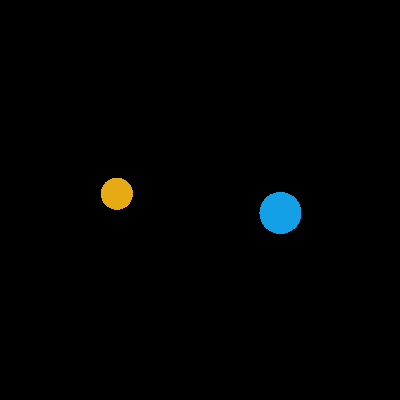
\includegraphics[width=0.43\linewidth]{figures/labels_0000_display.png}
\caption{Исходный синтетический кадр и карта меток двух шариков. Значения меток предназначены для машинной проверки.}
\end{figure}
\begin{figure}[htbp]\centering
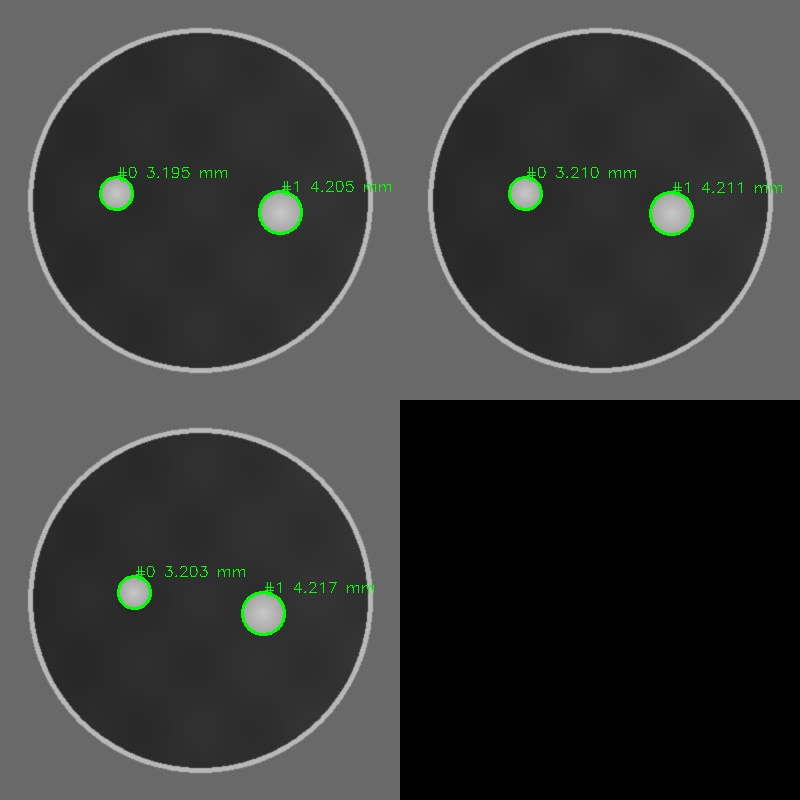
\includegraphics[width=0.70\linewidth]{figures/preview_sheet.jpg}
\caption{Контрольные кадры с найденными окружностями, идентификаторами и измеренными диаметрами.}
\end{figure}
\begin{figure}[htbp]\centering
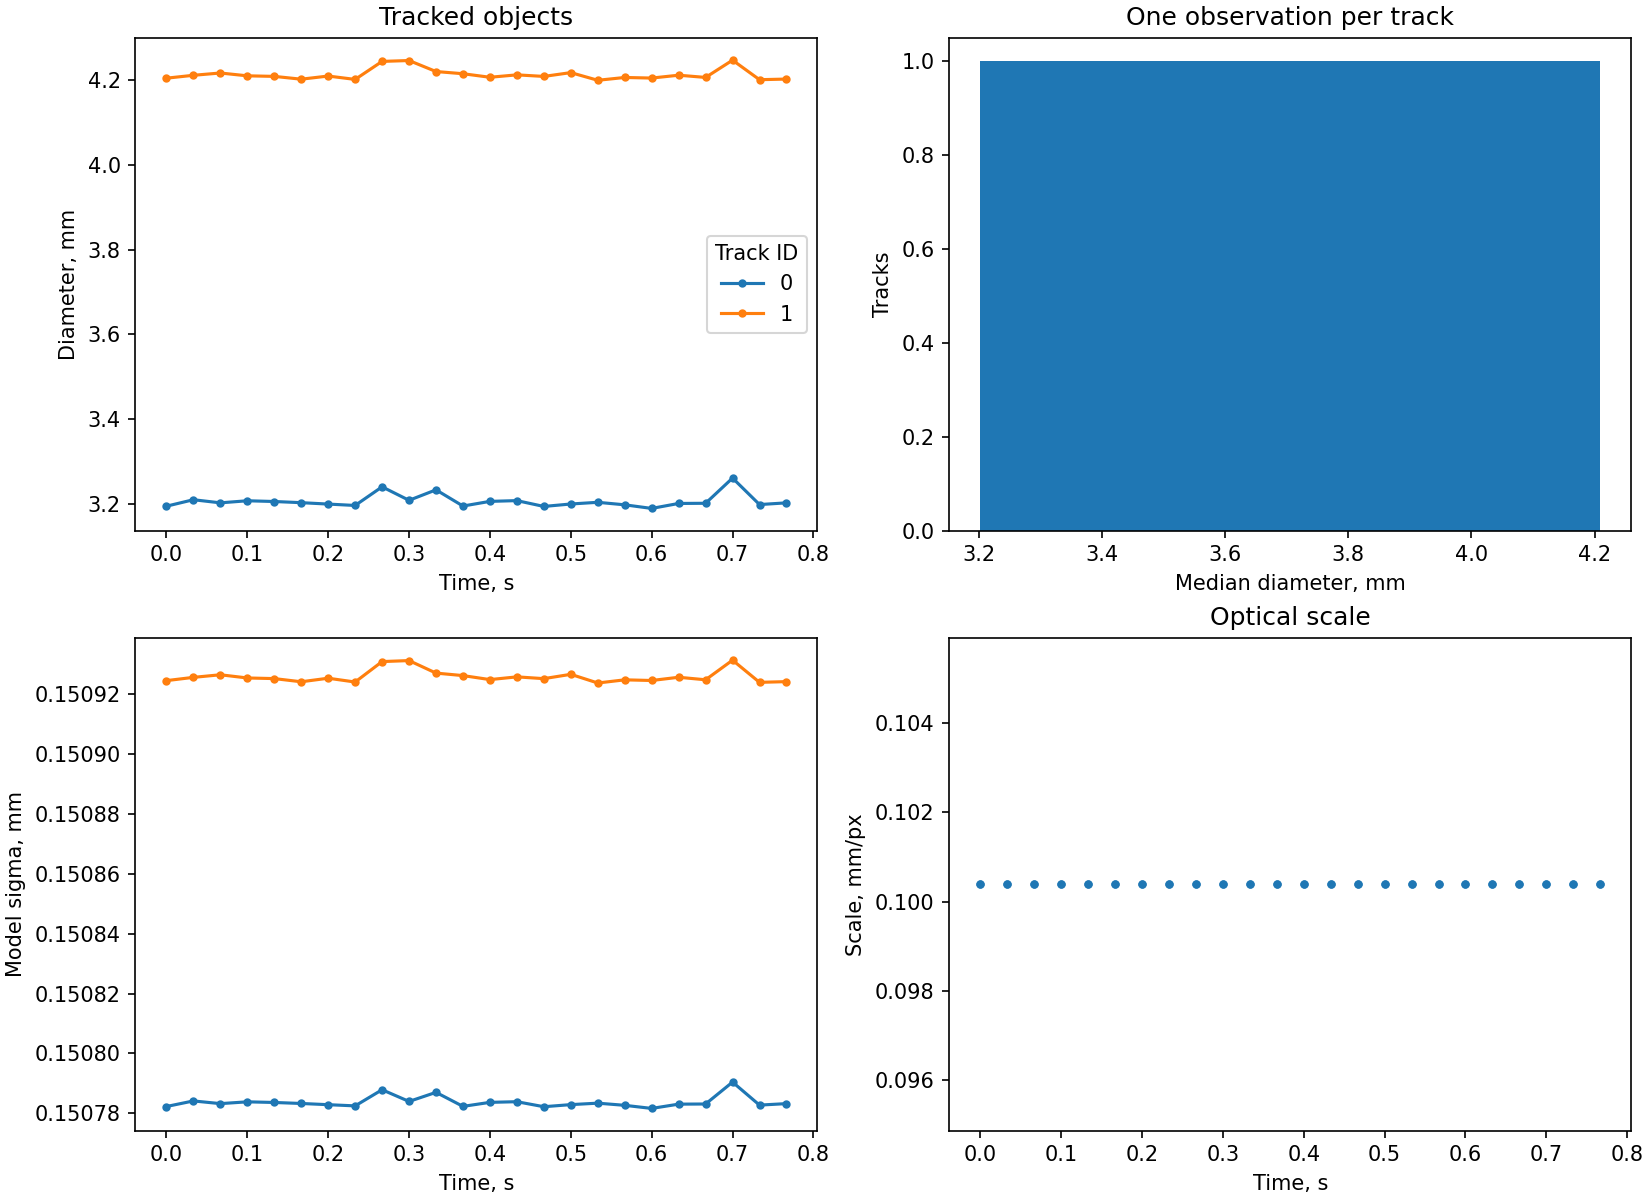
\includegraphics[width=\linewidth]{figures/series_plots.png}
\caption{Динамика диаметра, распределение медиан траекторий, модельная неопределённость и масштаб. Две траектории недостаточны для вывода о производственном распределении.}
\end{figure}
\clearpage
\section{Методика экспериментальной верификации}
Проверка на стенде должна начинаться с фиксации камеры, объектива, разрешения, освещения, экспозиции, положения оптической оси и геометрии наблюдения. Калибровочный объект регистрируется в той же оптической среде и плоскости, что и измеряемые шарики. Серии при иной глубине или уровне хладагента проверяются отдельно. Сохранение прежней ширины кадра является необходимым программным условием применения калибровки, но само по себе не подтверждает неизменность оптики.

Для эталона с независимым диаметром $D_{\mathrm{ref}}$ определяются смещение $\overline{\widehat d}-D_{\mathrm{ref}}$, разброс повторных измерений и зависимость ошибки от положения в кадре. Нужны серии с неподвижным и движущимся объектом, двумя шариками одновременно, бликами и частичными перекрытиями. Точность эталона и метод его независимого измерения фиксируются в протоколе. Повторные кадры одного эталона оценивают повторяемость; межсерийные изменения оптики требуют отдельных регистраций.

Для распределения размеров единицей наблюдения принимается подтверждённый физический шарик. Медиана диаметра по траектории уменьшает влияние повторных кадров, однако фрагменты траекторий необходимо проверять на повторный учёт одного шарика. Допустимый диапазон размеров и критерии брака определяются до обработки экспериментальной серии. Универсальная численная погрешность $\pm\Delta d$ к настоящей редакции не установлена.

\section{Выводы по разделу}
Разработанный программный контур выполняет измерение и сопровождение нескольких круговых объектов, использует сохранённую скалярную калибровку и формирует таблицы, графики и протокол обработки. Синтетическая проверка выявила ограничения при деформации и изменении масштаба. Она также подтвердила выполнение экспорта и сопровождение объектов в выбранных коротких сценах.

На следующем этапе я дополню раздел схемой монтажа, настройками стенда и материалами опробования камеры, проведу эталонную серию и обработаю изображения шариков в рабочей среде. По этим данным будут определены экспериментальная погрешность и распределение размеров; протоколы измерений войдут в окончательную редакцию. Результаты производительности макета и верификация тепловой модели относятся к отдельным разделам итогового отчёта.

\appendix
\section{Воспроизведение обработки}
\small
Точка запуска: \path{Mashine_Vision_Balls/run_analysis.py}. Синтетическая проверка выполняется с параметрами \texttt{--simulate-check}, \texttt{--simulation-seed 900}, \texttt{--simulation-frames 24}, \texttt{--simulation-output} и путём к новой пустой папке. Проверочные артефакты находятся в каталогах \path{output/simulation_holdout_900_20260930} и \path{output/simulation_holdout_901_20260930}. Файлы \texttt{validation.json} содержат метрики и хеши исходников; \texttt{truth.json} содержит разметку сцены. Выход анализатора включает \texttt{measurements.csv}, \texttt{tracks.csv}, \texttt{frames.csv}, \texttt{summary.json}, \texttt{run.json}, графики и контрольные кадры. Установка зависимостей определяется файлом \texttt{requirements.txt}; версии среды конкретной серии сохраняются в её протоколе.

\begin{thebibliography}{99}
\bibitem{tz} Техническое задание и календарный план НИР. Локальный документ: \path{ТЗ_НИР_Литвак_final version.docx}. Приложения № 1 и № 2 к договору, 2026.
\bibitem{code} Исходный код проекта Mashine\_Vision\_Balls: \path{run_analysis.py}; модули \path{series_analysis.py}, \texttt{simulation.py}, \texttt{pipeline.py}, \path{cv_geometry.py}, \texttt{reporting.py}. Версия, использованная при подготовке раздела: 30.09.2026. Исходники: \href{https://github.com/TryDotAtwo/Mashine_Vision_Balls/tree/3c97c4a92111cc8732bf2266364be1cae658515d/python_analysis}{GitHub, пакетный анализ и ClickHouse}; commit \texttt{3c97c4a}.
\bibitem{mathcode} Модуль \path{src/mvb/experiment_math.py}: функции пересчёта диаметра по геометрии и опорному объекту. Версия, использованная при подготовке раздела: 30.09.2026.
\bibitem{docs} Документация Mashine\_Vision\_Balls: \texttt{README.md}, \path{PURCHASE_SPEC_RU.md}, \path{UNCERTAINTY_METHOD_RU.md}, \path{PROJECT_MEMORY.md}. Состав закупки подтверждён отдельными счетами и перепиской.
\bibitem{tests} Модульные тесты Mashine\_Vision\_Balls. Команда: \texttt{py -3 -m unittest discover -s tests -v}. Результат 30.09.2026: 21 тест, OK, включая четыре теста локального ClickHouse.
\bibitem{simulation} Методика и протоколы синтетической проверки: \path{SIMULATION_METHOD_RU.md}; \texttt{simulation.py}; \texttt{validation.json}, seed 900 и 901, 30.09.2026. Источники модели: препринт ОИЯИ P18-2024-60, уравнения (5), (13), таблица П1; Gauthier A. et al. Self-propelled inverse Leidenfrost droplets, arXiv:1901.04218, уравнение (5).
\bibitem{cameraorder} ООО «МКОИ». Счёт № 382 от 26.09.2025: камера Daheng MER2-231-41GM, кабель I/O и крепление. Локальный файл \path{382_OIYAI-RAN.pdf}.
\bibitem{opticsorder} ООО «Компания «Азимут Фотоникс». Счёт № 15022 от 20.11.2025: объектив, кольца, освещение, контроллер, питание и кронштейны. Локальная копия в \path{Mashine_Vision_Balls/data/documents}.
\bibitem{equipmentupd} ООО «Компания «Азимут Фотоникс». УПД № 78 от 19.02.2026 к счёту № 15022. Копия приложена к письму А. Герасимовой от 30.03.2026. Дата приёмки получателем не заполнена.
\bibitem{equipmentmail} Переписка И. Л. Литвака с «Азимут Фотоникс», тема «Подбор объектива на камеру»: запрос 12.11.2025; согласование комплектации 20.11.2025; подтверждение оплаты 10.12.2025; уточнение поставки кабеля 20.04.2026. Реестр писем сохранён в \path{sources/equipment_evidence.md}.
\bibitem{daheng} DAHENG IMAGING. MER2-231-41GM. Паспортные характеристики. \url{https://en.daheng-imaging.com/show-104-1901-1.html}. Проверено 30.09.2026.
\bibitem{manualv2} Литвак И. Л. Руководство по эксперименту и обработке видеозаписей шариков. Версия 2.1 от 30.09.2026. Исходник: \path{stand_manual_v2.tex}. Обновлённая редакция инструкции от 02.04.2026; полный текст включён в приложение.
\bibitem{clickhouse} ClickHouse. HTTP interface. Официальная документация. \url{https://clickhouse.com/docs/interfaces/http}. Проверено 30.09.2026.
\end{thebibliography}
\clearpage
\section{Руководство по эксперименту, версия 2.1}
Полный текст новой редакции приведён на следующих страницах. Нумерация внутри руководства сохранена; это самостоятельный документ для работы на стенде.
\clearpage\newgeometry{margin=0mm}\pagestyle{empty}
\noindent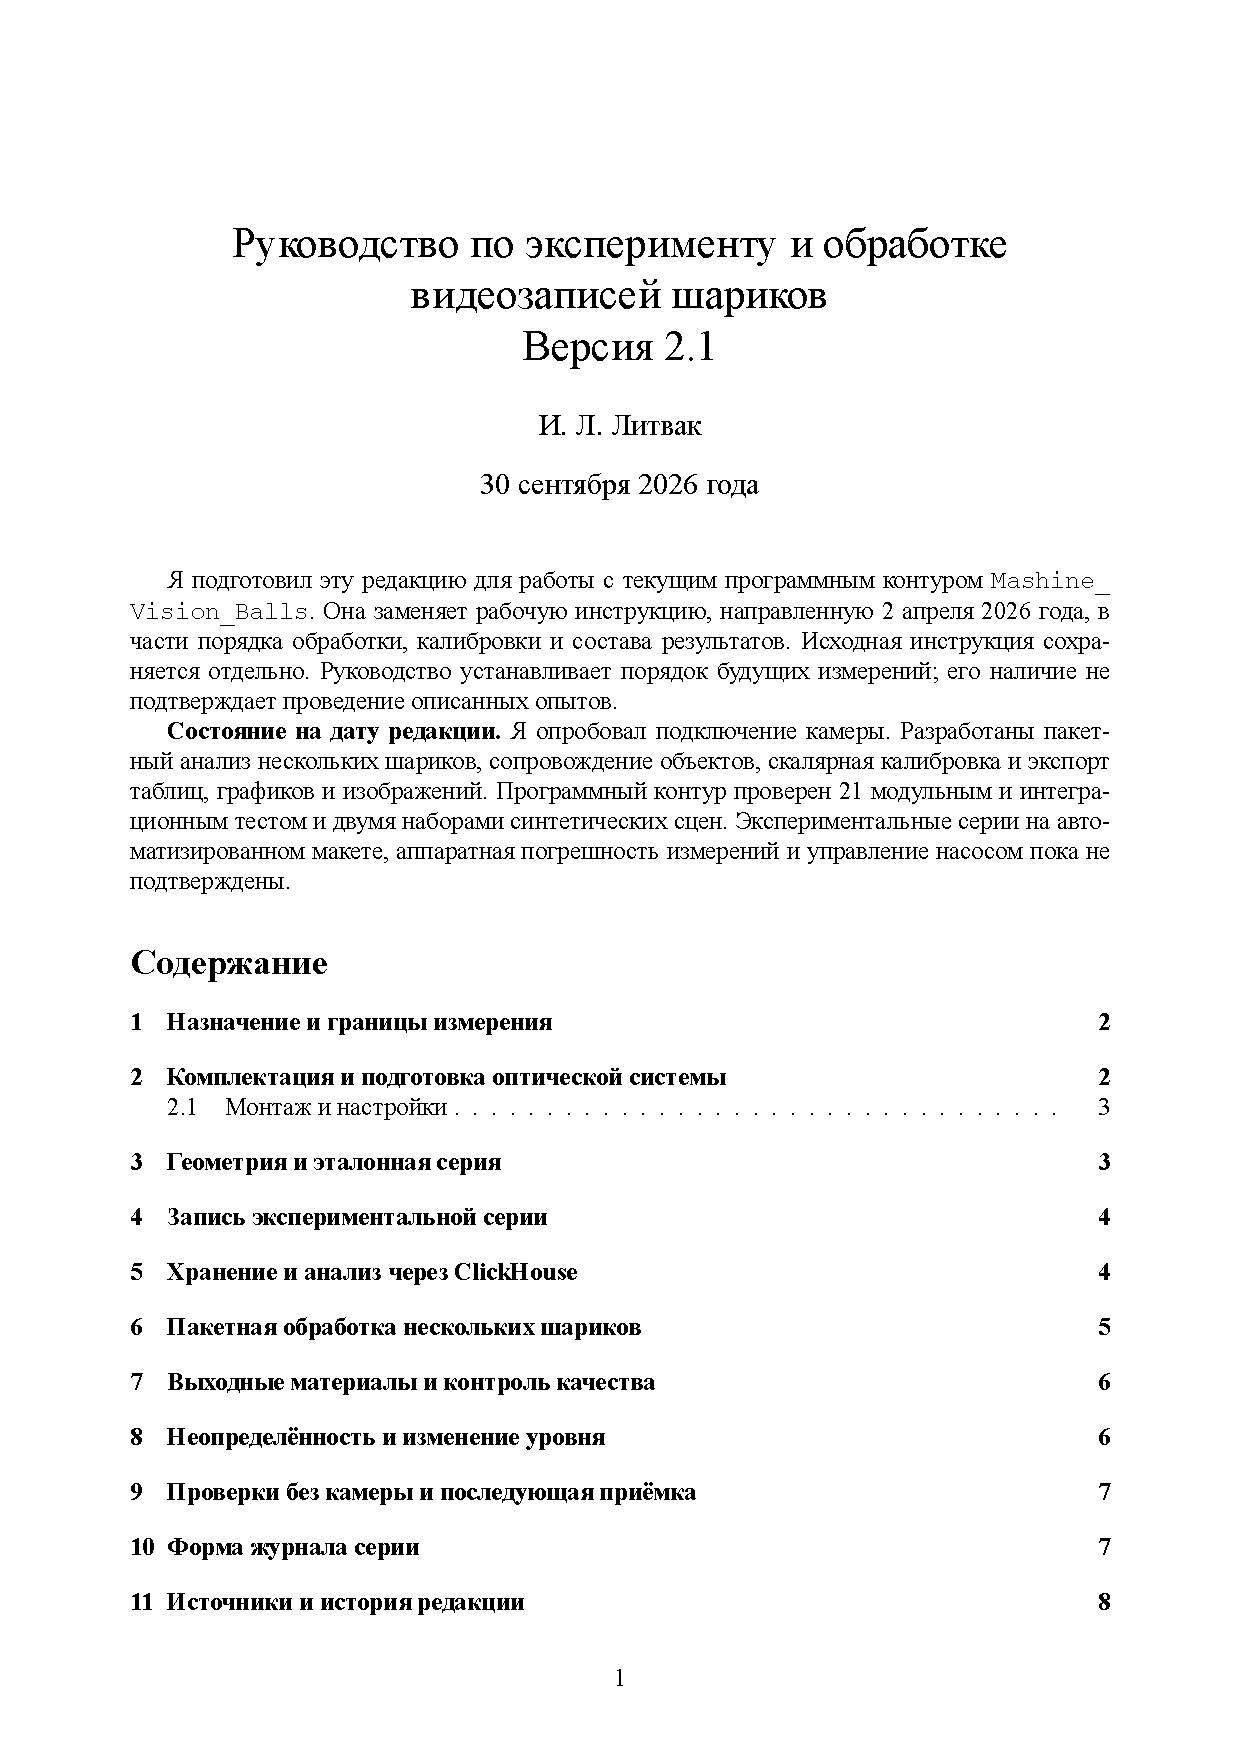
\includegraphics[page=1,width=0.97\paperwidth,height=0.97\paperheight,keepaspectratio]{stand_manual_v2.pdf}\clearpage
\noindent\includegraphics[page=2,width=0.97\paperwidth,height=0.97\paperheight,keepaspectratio]{stand_manual_v2.pdf}\clearpage
\noindent\includegraphics[page=3,width=0.97\paperwidth,height=0.97\paperheight,keepaspectratio]{stand_manual_v2.pdf}\clearpage
\noindent\includegraphics[page=4,width=0.97\paperwidth,height=0.97\paperheight,keepaspectratio]{stand_manual_v2.pdf}\clearpage
\noindent\includegraphics[page=5,width=0.97\paperwidth,height=0.97\paperheight,keepaspectratio]{stand_manual_v2.pdf}\clearpage
\noindent\includegraphics[page=6,width=0.97\paperwidth,height=0.97\paperheight,keepaspectratio]{stand_manual_v2.pdf}\clearpage
\noindent\includegraphics[page=7,width=0.97\paperwidth,height=0.97\paperheight,keepaspectratio]{stand_manual_v2.pdf}\clearpage
\noindent\includegraphics[page=8,width=0.97\paperwidth,height=0.97\paperheight,keepaspectratio]{stand_manual_v2.pdf}\clearpage\restoregeometry
\end{document}